
%% bare_jrnl.tex
%% V1.4a
%% 2014/09/17
%% by Michael Shell
%% see http://www.michaelshell.org/
%% for current contact information.
%%
%% This is a skeleton file demonstrating the use of IEEEtran.cls
%% (requires IEEEtran.cls version 1.8a or later) with an IEEE
%% journal paper.
%%
%% Support sites:
%% http://www.michaelshell.org/tex/ieeetran/
%% http://www.ctan.org/tex-archive/macros/latex/contrib/IEEEtran/
%% and
%% http://www.ieee.org/

%%*************************************************************************
%% Legal Notice:
%% This code is offered as-is without any warranty either expressed or
%% implied; without even the implied warranty of MERCHANTABILITY or
%% FITNESS FOR A PARTICULAR PURPOSE! 
%% User assumes all risk.
%% In no event shall IEEE or any contributor to this code be liable for
%% any damages or losses, including, but not limited to, incidental,
%% consequential, or any other damages, resulting from the use or misuse
%% of any information contained here.
%%
%% All comments are the opinions of their respective authors and are not
%% necessarily endorsed by the IEEE.
%%
%% This work is distributed under the LaTeX Project Public License (LPPL)
%% ( http://www.latex-project.org/ ) version 1.3, and may be freely used,
%% distributed and modified. A copy of the LPPL, version 1.3, is included
%% in the base LaTeX documentation of all distributions of LaTeX released
%% 2003/12/01 or later.
%% Retain all contribution notices and credits.
%% ** Modified files should be clearly indicated as such, including  **
%% ** renaming them and changing author support contact information. **
%%
%% File list of work: IEEEtran.cls, IEEEtran_HOWTO.pdf, bare_adv.tex,
%%                    bare_conf.tex, bare_jrnl.tex, bare_conf_compsoc.tex,
%%                    bare_jrnl_compsoc.tex, bare_jrnl_transmag.tex
%%*************************************************************************


% *** Authors should verify (and, if needed, correct) their LaTeX system  ***
% *** with the testflow diagnostic prior to trusting their LaTeX platform ***
% *** with production work. IEEE's font choices and paper sizes can       ***
% *** trigger bugs that do not appear when using other class files.       ***                          ***
% The testflow support page is at:
% http://www.michaelshell.org/tex/testflow/



\documentclass[journal]{IEEEtran}
%
% If IEEEtran.cls has not been installed into the LaTeX system files,
% manually specify the path to it like:
% \documentclass[journal]{../sty/IEEEtran}





% Some very useful LaTeX packages include:
% (uncomment the ones you want to load)


% *** MISC UTILITY PACKAGES ***
%
%\usepackage{ifpdf}
% Heiko Oberdiek's ifpdf.sty is very useful if you need conditional
% compilation based on whether the output is pdf or dvi.
% usage:
% \ifpdf
%   % pdf code
% \else
%   % dvi code
% \fi
% The latest version of ifpdf.sty can be obtained from:
% http://www.ctan.org/tex-archive/macros/latex/contrib/oberdiek/
% Also, note that IEEEtran.cls V1.7 and later provides a builtin
% \ifCLASSINFOpdf conditional that works the same way.
% When switching from latex to pdflatex and vice-versa, the compiler may
% have to be run twice to clear warning/error messages.






% *** CITATION PACKAGES ***
%
%\usepackage{cite}
% cite.sty was written by Donald Arseneau
% V1.6 and later of IEEEtran pre-defines the format of the cite.sty package
% \cite{} output to follow that of IEEE. Loading the cite package will
% result in citation numbers being automatically sorted and properly
% "compressed/ranged". e.g., [1], [9], [2], [7], [5], [6] without using
% cite.sty will become [1], [2], [5]--[7], [9] using cite.sty. cite.sty's
% \cite will automatically add leading space, if needed. Use cite.sty's
% noadjust option (cite.sty V3.8 and later) if you want to turn this off
% such as if a citation ever needs to be enclosed in parenthesis.
% cite.sty is already installed on most LaTeX systems. Be sure and use
% version 5.0 (2009-03-20) and later if using hyperref.sty.
% The latest version can be obtained at:
% http://www.ctan.org/tex-archive/macros/latex/contrib/cite/
% The documentation is contained in the cite.sty file itself.






% *** GRAPHICS RELATED PACKAGES ***
%
\ifCLASSINFOpdf
  % \usepackage[pdftex]{graphicx}
  % declare the path(s) where your graphic files are
  % \graphicspath{{../pdf/}{../jpeg/}}
  % and their extensions so you won't have to specify these with
  % every instance of \includegraphics
  % \DeclareGraphicsExtensions{.pdf,.jpeg,.png}
\else
  % or other class option (dvipsone, dvipdf, if not using dvips). graphicx
  % will default to the driver specified in the system graphics.cfg if no
  % driver is specified.
  % \usepackage[dvips]{graphicx}
  % declare the path(s) where your graphic files are
  % \graphicspath{{../eps/}}
  % and their extensions so you won't have to specify these with
  % every instance of \includegraphics
  % \DeclareGraphicsExtensions{.eps}
\fi
% graphicx was written by David Carlisle and Sebastian Rahtz. It is
% required if you want graphics, photos, etc. graphicx.sty is already
% installed on most LaTeX systems. The latest version and documentation
% can be obtained at: 
% http://www.ctan.org/tex-archive/macros/latex/required/graphics/
% Another good source of documentation is "Using Imported Graphics in
% LaTeX2e" by Keith Reckdahl which can be found at:
% http://www.ctan.org/tex-archive/info/epslatex/
%
% latex, and pdflatex in dvi mode, support graphics in encapsulated
% postscript (.eps) format. pdflatex in pdf mode supports graphics
% in .pdf, .jpeg, .png and .mps (metapost) formats. Users should ensure
% that all non-photo figures use a vector format (.eps, .pdf, .mps) and
% not a bitmapped formats (.jpeg, .png). IEEE frowns on bitmapped formats
% which can result in "jaggedy"/blurry rendering of lines and letters as
% well as large increases in file sizes.
%
% You can find documentation about the pdfTeX application at:
% http://www.tug.org/applications/pdftex





% *** MATH PACKAGES ***
%
%\usepackage[cmex10]{amsmath}
% A popular package from the American Mathematical Society that provides
% many useful and powerful commands for dealing with mathematics. If using
% it, be sure to load this package with the cmex10 option to ensure that
% only type 1 fonts will utilized at all point sizes. Without this option,
% it is possible that some math symbols, particularly those within
% footnotes, will be rendered in bitmap form which will result in a
% document that can not be IEEE Xplore compliant!
%
% Also, note that the amsmath package sets \interdisplaylinepenalty to 10000
% thus preventing page breaks from occurring within multiline equations. Use:
%\interdisplaylinepenalty=2500
% after loading amsmath to restore such page breaks as IEEEtran.cls normally
% does. amsmath.sty is already installed on most LaTeX systems. The latest
% version and documentation can be obtained at:
% http://www.ctan.org/tex-archive/macros/latex/required/amslatex/math/





% *** SPECIALIZED LIST PACKAGES ***
%
%\usepackage{algorithmic}
% algorithmic.sty was written by Peter Williams and Rogerio Brito.
% This package provides an algorithmic environment fo describing algorithms.
% You can use the algorithmic environment in-text or within a figure
% environment to provide for a floating algorithm. Do NOT use the algorithm
% floating environment provided by algorithm.sty (by the same authors) or
% algorithm2e.sty (by Christophe Fiorio) as IEEE does not use dedicated
% algorithm float types and packages that provide these will not provide
% correct IEEE style captions. The latest version and documentation of
% algorithmic.sty can be obtained at:
% http://www.ctan.org/tex-archive/macros/latex/contrib/algorithms/
% There is also a support site at:
% http://algorithms.berlios.de/index.html
% Also of interest may be the (relatively newer and more customizable)
% algorithmicx.sty package by Szasz Janos:
% http://www.ctan.org/tex-archive/macros/latex/contrib/algorithmicx/




% *** ALIGNMENT PACKAGES ***
%
%\usepackage{array}
% Frank Mittelbach's and David Carlisle's array.sty patches and improves
% the standard LaTeX2e array and tabular environments to provide better
% appearance and additional user controls. As the default LaTeX2e table
% generation code is lacking to the point of almost being broken with
% respect to the quality of the end results, all users are strongly
% advised to use an enhanced (at the very least that provided by array.sty)
% set of table tools. array.sty is already installed on most systems. The
% latest version and documentation can be obtained at:
% http://www.ctan.org/tex-archive/macros/latex/required/tools/


% IEEEtran contains the IEEEeqnarray family of commands that can be used to
% generate multiline equations as well as matrices, tables, etc., of high
% quality.




% *** SUBFIGURE PACKAGES ***
%\ifCLASSOPTIONcompsoc
%  \usepackage[caption=false,font=normalsize,labelfont=sf,textfont=sf]{subfig}
%\else
%  \usepackage[caption=false,font=footnotesize]{subfig}
%\fi
% subfig.sty, written by Steven Douglas Cochran, is the modern replacement
% for subfigure.sty, the latter of which is no longer maintained and is
% incompatible with some LaTeX packages including fixltx2e. However,
% subfig.sty requires and automatically loads Axel Sommerfeldt's caption.sty
% which will override IEEEtran.cls' handling of captions and this will result
% in non-IEEE style figure/table captions. To prevent this problem, be sure
% and invoke subfig.sty's "caption=false" package option (available since
% subfig.sty version 1.3, 2005/06/28) as this is will preserve IEEEtran.cls
% handling of captions.
% Note that the Computer Society format requires a larger sans serif font
% than the serif footnote size font used in traditional IEEE formatting
% and thus the need to invoke different subfig.sty package options depending
% on whether compsoc mode has been enabled.
%
% The latest version and documentation of subfig.sty can be obtained at:
% http://www.ctan.org/tex-archive/macros/latex/contrib/subfig/




% *** FLOAT PACKAGES ***
%
%\usepackage{fixltx2e}
% fixltx2e, the successor to the earlier fix2col.sty, was written by
% Frank Mittelbach and David Carlisle. This package corrects a few problems
% in the LaTeX2e kernel, the most notable of which is that in current
% LaTeX2e releases, the ordering of single and double column floats is not
% guaranteed to be preserved. Thus, an unpatched LaTeX2e can allow a
% single column figure to be placed prior to an earlier double column
% figure. The latest version and documentation can be found at:
% http://www.ctan.org/tex-archive/macros/latex/base/


%\usepackage{stfloats}
% stfloats.sty was written by Sigitas Tolusis. This package gives LaTeX2e
% the ability to do double column floats at the bottom of the page as well
% as the top. (e.g., "\begin{figure*}[!b]" is not normally possible in
% LaTeX2e). It also provides a command:
%\fnbelowfloat
% to enable the placement of footnotes below bottom floats (the standard
% LaTeX2e kernel puts them above bottom floats). This is an invasive package
% which rewrites many portions of the LaTeX2e float routines. It may not work
% with other packages that modify the LaTeX2e float routines. The latest
% version and documentation can be obtained at:
% http://www.ctan.org/tex-archive/macros/latex/contrib/sttools/
% Do not use the stfloats baselinefloat ability as IEEE does not allow
% \baselineskip to stretch. Authors submitting work to the IEEE should note
% that IEEE rarely uses double column equations and that authors should try
% to avoid such use. Do not be tempted to use the cuted.sty or midfloat.sty
% packages (also by Sigitas Tolusis) as IEEE does not format its papers in
% such ways.
% Do not attempt to use stfloats with fixltx2e as they are incompatible.
% Instead, use Morten Hogholm'a dblfloatfix which combines the features
% of both fixltx2e and stfloats:
%
% \usepackage{dblfloatfix}
% The latest version can be found at:
% http://www.ctan.org/tex-archive/macros/latex/contrib/dblfloatfix/




%\ifCLASSOPTIONcaptionsoff
%  \usepackage[nomarkers]{endfloat}
% \let\MYoriglatexcaption\caption
% \renewcommand{\caption}[2][\relax]{\MYoriglatexcaption[#2]{#2}}
%\fi
% endfloat.sty was written by James Darrell McCauley, Jeff Goldberg and 
% Axel Sommerfeldt. This package may be useful when used in conjunction with 
% IEEEtran.cls'  captionsoff option. Some IEEE journals/societies require that
% submissions have lists of figures/tables at the end of the paper and that
% figures/tables without any captions are placed on a page by themselves at
% the end of the document. If needed, the draftcls IEEEtran class option or
% \CLASSINPUTbaselinestretch interface can be used to increase the line
% spacing as well. Be sure and use the nomarkers option of endfloat to
% prevent endfloat from "marking" where the figures would have been placed
% in the text. The two hack lines of code above are a slight modification of
% that suggested by in the endfloat docs (section 8.4.1) to ensure that
% the full captions always appear in the list of figures/tables - even if
% the user used the short optional argument of \caption[]{}.
% IEEE papers do not typically make use of \caption[]'s optional argument,
% so this should not be an issue. A similar trick can be used to disable
% captions of packages such as subfig.sty that lack options to turn off
% the subcaptions:
% For subfig.sty:
% \let\MYorigsubfloat\subfloat
% \renewcommand{\subfloat}[2][\relax]{\MYorigsubfloat[]{#2}}
% However, the above trick will not work if both optional arguments of
% the \subfloat command are used. Furthermore, there needs to be a
% description of each subfigure *somewhere* and endfloat does not add
% subfigure captions to its list of figures. Thus, the best approach is to
% avoid the use of subfigure captions (many IEEE journals avoid them anyway)
% and instead reference/explain all the subfigures within the main caption.
% The latest version of endfloat.sty and its documentation can obtained at:
% http://www.ctan.org/tex-archive/macros/latex/contrib/endfloat/
%
% The IEEEtran \ifCLASSOPTIONcaptionsoff conditional can also be used
% later in the document, say, to conditionally put the References on a 
% page by themselves.




% *** PDF, URL AND HYPERLINK PACKAGES ***
%
%\usepackage{url}
% url.sty was written by Donald Arseneau. It provides better support for
% handling and breaking URLs. url.sty is already installed on most LaTeX
% systems. The latest version and documentation can be obtained at:
% http://www.ctan.org/tex-archive/macros/latex/contrib/url/
% Basically, \url{my_url_here}.

\usepackage{color}
\usepackage{listings,comment}

\lstdefinelanguage{NeoIDL}{
  sensitive = true, 
  keywords = {module, service, import, struct, path},
 %basicstyle=\normalfont\ttfamily,
    numbers=left,
    numberstyle=\scriptsize,
    stepnumber=1,
    numbersep=8pt,
    showstringspaces=false,
    breaklines=true,
    frame=lines,
    %backgroundcolor=\color{background}
}

% *** Do not adjust lengths that control margins, column widths, etc. ***
% *** Do not use packages that alter fonts (such as pslatex).         ***
% There should be no need to do such things with IEEEtran.cls V1.6 and later.
% (Unless specifically asked to do so by the journal or conference you plan
% to submit to, of course. )


% correct bad hyphenation here
\hyphenation{op-tical net-works semi-conduc-tor}

\usepackage[utf8]{inputenc}
\newcommand{\neoidl}{NeoIDL}

\begin{document}
%
% paper title
% Titles are generally capitalized except for words such as a, an, and, as,
% at, but, by, for, in, nor, of, on, or, the, to and up, which are usually
% not capitalized unless they are the first or last word of the title.
% Linebreaks \\ can be used within to get better formatting as desired.
% Do not put math or special symbols in the title.
\title{Contratos REST robustos e leves: uma abordagem em Design-by-Contract
com NeoIDL}


%
%
% author names and IEEE memberships
% note positions of commas and nonbreaking spaces ( ~ ) LaTeX will not break
% a structure at a ~ so this keeps an author's name from being broken across
% two lines.
% use \thanks{} to gain access to the first footnote area
% a separate \thanks must be used for each paragraph as LaTeX2e's \thanks
% was not built to handle multiple paragraphs
%

\author{Lucas F. Lima,~\IEEEmembership{Mestrando,~UnB,}
        Rodrigo Bonifácio de Almeida,~\IEEEmembership{Professor,~UnB,}
        Edna Dias Canedo,~\IEEEmembership{Professor,~UnB}% <-this % stops a
        % space
}

% note the % following the last \IEEEmembership and also \thanks - 
% these prevent an unwanted space from occurring between the last author name
% and the end of the author line. i.e., if you had this:
% 
% \author{....lastname \thanks{...} \thanks{...} }
%                     ^------------^------------^----Do not want these spaces!
%
% a space would be appended to the last name and could cause every name on that
% line to be shifted left slightly. This is one of those "LaTeX things". For
% instance, "\textbf{A} \textbf{B}" will typeset as "A B" not "AB". To get
% "AB" then you have to do: "\textbf{A}\textbf{B}"
% \thanks is no different in this regard, so shield the last } of each \thanks
% that ends a line with a % and do not let a space in before the next \thanks.
% Spaces after \IEEEmembership other than the last one are OK (and needed) as
% you are supposed to have spaces between the names. For what it is worth,
% this is a minor point as most people would not even notice if the said evil
% space somehow managed to creep in.



% The paper headers
\markboth{Workshop da Pós-Graduação em Computação (WPOS 2015), Outubro 2015}%
{Shell \MakeLowercase{\textit{et al.}}: Bare Demo of IEEEtran.cls for Journals}
% The only time the second header will appear is for the odd numbered pages
% after the title page when using the twoside option.
% 
% *** Note that you probably will NOT want to include the author's ***
% *** name in the headers of peer review papers.                   ***
% You can use \ifCLASSOPTIONpeerreview for conditional compilation here if
% you desire.




% If you want to put a publisher's ID mark on the page you can do it like
% this:
%\IEEEpubid{0000--0000/00\$00.00~\copyright~2014 IEEE}
% Remember, if you use this you must call \IEEEpubidadjcol in the second
% column for its text to clear the IEEEpubid mark.



% use for special paper notices
%\IEEEspecialpapernotice{(Invited Paper)}




% make the title area
\maketitle

% As a general rule, do not put math, special symbols or citations
% in the abstract or keywords.
\begin{abstract}
O trabalho de pesquisa de mestrado, sumarizado neste artigo, objetiva
  fortalecer a especificação de contratos para soluções concebidas sob o
  paradigma de computação orientada a serviços. A robustez é buscada por meio de
  construções que agregam \textit{Design-by-Contract} à linguagem \neoidl{}, de
  modo que os serviços especificados assegurem as pós-condições, desde que
  satisfeitas suas pré-condições.
  A proposta será submetida a validação empírica, verificando regras de
  transformações em um novo plugin para a \neoidl{}.
\end{abstract}

% Note that keywords are not normally used for peerreview papers.
\begin{IEEEkeywords}
\neoidl{}, Desing-by-contract, REST, SOC, DSL, Contract first.
\end{IEEEkeywords}






% For peer review papers, you can put extra information on the cover
% page as needed:
% \ifCLASSOPTIONpeerreview
% \begin{center} \bfseries EDICS Category: 3-BBND \end{center}
% \fi
%
% For peerreview papers, this IEEEtran command inserts a page break and
% creates the second title. It will be ignored for other modes.
\IEEEpeerreviewmaketitle

\section{Introdução e Caracterização do Problema}\label{sec:introducao}

A computação orientada a serviços ( \emph{Service-oriented computing, SOC)} tem
se mostrado uma solução de \textit{design} de \textit{software} que favorece o
alinhamento às mudanças constantes e urgentes nas insituições
\cite{chen2008towards}. Os benefícios de SOC estão diretamente relacionados ao
baixo acoplamento dos serviços que compõem a solução, de forma que as partes
(nesse caso serviços) possam ser substituídas e evoluídas facilmente, ou ainda
rearranjadas em novas composições. Contudo, para que isso seja possível, é
necessário que os serviços possuam contratos bem definidos e independentes da
implementação.

Por outro lado, as linguagens de especificação de contratos para SOA apresentam
algumas limitações. Por exemplo, a linguagem WSDL (\emph{Web-services
description language}) \cite{zur2005developing} é considerada uma solução
verbosa que desestimula a abordagem \textit{Contract First}. Por essa razão,
especificações WSDL são usualmente derivadas a partir de anotações em código
fonte.
Além disso, os conceitos descritos em contratos na linguagem WSDL não são
diretamente mapeados aos elementos que compõem as interfaces do estilo
arquitetural REST (\emph{Representational State Transfer}).
Outras alternativas para REST, como Swagger e
RAML\footnote{http://raml.org/spec.html}, usam linguagens de propósito geral (em
particular JSON) adaptadas para especificação de contratos. Ainda que façam uso
de contratos mais sucintos que WSDL, essas linguagens não se
beneficiam da clareza típica das linguagens específicas para esse fim (como IDLs CORBA) e não oferecem
mecanismos semânticos de extensibilidade e modularidade.

Com o objetivo de mitigar esses problemas, a linguagem \neoidl foi proposta
para simplificar a especificação de serviços REST com mecanismos de modularização,
suporte a anotações, herança em tipos de dados definidos pelo desenvolvedor, e
uma sintaxe simples e concisa semelhante às \textit{Interface Description
Languages} -- IDLs -- presentes em \textit{Apache Thrift}\texttrademark e
CORBA\texttrademark. Por outro lado, a \neoidl, da mesma forma que WSDL, Swagger
e RAML não oferece construções para especificação de contratos formais de
comportamento como os presentes em linguagens que suportam DBC (\emph{Design by
Contract})~\cite{meyer1992applying}, como JML, Spec\# e Eiffel.

Dessa forma, os objetivos dessa pesquisa envolvem inicialmente investigar o uso
de construções DBC no contexto da computação orientada a serviços e conduzir uma
revisão sistemática da literatura para identificar os principais trabalhos que
lidam com a relação entre DBC e SOC. Em seguida especificar e implementar novas
construções para a linguagem \neoidl, de tal forma que seja possível especificar
contratos mais precisos; além de definir regras de transformação das novas
construções \neoidl para diferentes tecnologias (como Twisted) que suportam a
implementação de serviços em REST.
Por fim, conduzir uma validação empírica da proposta usando uma abordagem mais
exploratória, possivelmente usando a estratégia \emph{pesquisa-ação}.




\section{Fundamentação Teórica}\label{sec:fundamentacao}

SOC é um estilo arquitetural cujo objetivo é prover baixo acoplamento por meio
da interação entre agentes de software, chamados de serviços
\cite{he2003service}. A chave para que a solução baseada em SOC tenha
custo-benefício favorável é o reuso, o qual somente é possível se os serviços
possuírem interfaces ubíquas, com semânticas genéricas e disponíveis para seus
consumidores. Usualmente, a comunicação com os serviços, e entre eles, é feita
por meio da troca de mensagens com uso de \textit{servi\c cos web}, que seguem
padrões abertos de comunicação e que atuam sobre o protocolo HTTP. SOAP e
REST~\cite{fielding2000fielding} s\~{a}o as tecnologias mais usadas para
implementa\c c\~{a}o de servi\c cos web, sendo que REST tem atra\'{i}do um maior
interesse nos \'{u}ltimos anos.

Entre os oito princípios para desenvolvimento SOA descritos
em~\cite{erl2008soa}, existe um especial interesse no \emph{contrato
padronizado} (\textit{Standardized Service Contract}), que sugere que serviços
de um mesmo inventário devem seguir os mesmos padrões de \textit{design}, de
modo a favorecer o reuso e composição. Este princípio prega a abordagem
\textit{Contract First}, em que a concepção do serviço parte da especificação do
contrato e não com a geração do contrato a partir código. \'{E} importante
destacar que n\~{a}o existe um padr\~{a}o para especificar contratos em REST, o
que motivou o desenho da \neoidl~\cite{bonifacio2015neoidl}, uma linguagem
espec\'{i}fica do dom\'{i}nio para especificação de contratos REST e que,
diferente das linguagens existents, prov\^{e} recursos de modularidade e herança
de tipos de dados customizados. Utilizando uma abordagem transformacional, a
\neoidl{} oferece suporte ferramental que gera c\'{o}digo fonte para diferentes
linguagens e plataformas REST, a partir de um conjunto de módulos \neoidl{} onde
são especificados os tipos de dados e os serviços.

A Figura \ref{lst:modulobasiconeo} apresenta um exemplo de módulo \neoidl{}
com a defini\c c\~{a}o de um tipo de dados \texttt{ItemDoCatalogo} e duas
opera\c c\~{o}es (chamadas de capacidades na terminologia REST):
\texttt{atualizarItem} (opera\c c\~{a}o do tipo POST associada ao
\emph{endpoint} \texttt{catalogo}) e \texttt{pesquisarItem} (opera\c c\~{a}o do
tipo GET, do mesmo \emph{endpoint}).


\begin{figure}[htb]
\begin{scriptsize}
\lstinputlisting[language=NeoIDL,firstnumber=1]{getCharactersDbc.tex}
\end{scriptsize}
\caption{Exemplo de um módulo escrito em \neoidl}
\label{lst:modulobasiconeo}
\end{figure}


Conforme mencionado, o suporte ferramental da \neoidl{} processa um conjunto de
módulos escritos na linguagem \neoidl{}, gerando o código com a estrutura para
implementação dos serviços descritos.
A versão atual do ambiente \neoidl{} suporta geração de códigos em Java e Python
para as plataformas \emph{neoCortex}\footnote{propriet\'{a}ria do Ex\'{e}rcito
Brasileiro} e \emph{Twisted}. Entretanto, esse ambiente é extensível por meio
da implementação de novos plugins~\cite{bonifacio2015neoidl}.


%% \begin{figure}[ht] \centering
%% 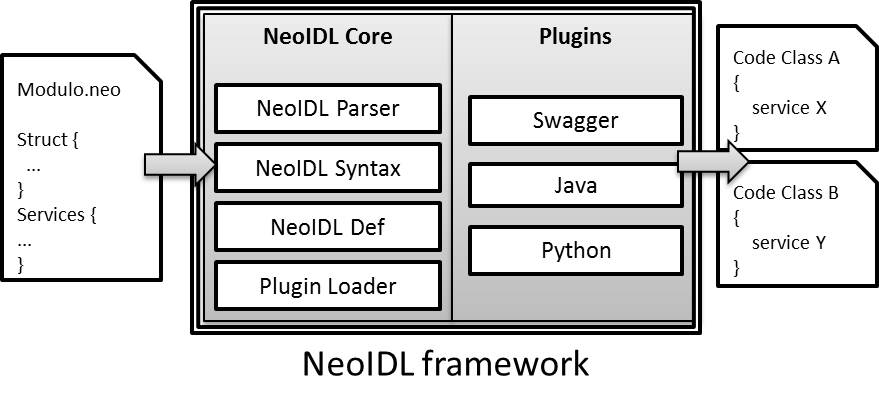
\includegraphics[width=.5\textwidth]{NeoIDLFrameworkArchtecture.jpg}
%% \caption{Entradas (lado esquerdo) e saídas (lado direito) do \textit{framework}
%% \neoidl}
%% \label{fig:NeoFrameArch}
%% \end{figure}

\emph{Limita\c c\~{a}o da \neoidl}. Atualmente a \neoidl{} permite apenas a
especifica\c c\~{a}o de \emph{weak contracts}, o que n\~{a}o permite estabelecer
obriga\c c\~{o}es entre fornecedores e clientes de servi\c cos. Esse tipo de
obriga\c c\~{a}o pode ser estabelecida com alguma t\'{e}cnica de
\emph{Design-by-contract}~\cite{meyer1992applying} (DBC) -- na qual o consumidor
e o fornecedor de servi\c cos firmam entre si um conjunto de garantias. Em um
contexto mais simples, de um lado o consumidor deve garantir que, antes da
chamada a um servi\c co (ou um m\'{e}todo de uma classe), os parâmetros de
entrada devem ser respeitados (essas garantias s\~{a}o denominadas de
pré-condições). Do outro lado, o fornecedor deve garantir que, uma vez
respeitadas as pré-condições, as propriedades relacionadas ao sucesso da
execução (pós-condições) s\~{a}o preservadas. DBC tem o objetivo de aumentar a
robustez do sistema e tem na linguagem Eiffel \cite{meyer1991eiffel} um de seus
precursores. O uso de DBC na concepção de sistemas, segundo
\cite{EiffelDBC:2012} é uma abordagem sistemática que tende a reduzir a
quantidade de erros observados nos sistemas.
Mais recentemente, algumas t\'{e}cnicas de \emph{design-by-contract} foram
especificadas e implementadas para outras linguagens de programa\c c\~{a}o, como
JML para a linguagem Java~\cite{leavens} e \texttt{Spec\#} para a linguagem
\texttt{C\#} (e demais linguagens da plataforma .NET)~\cite{barthe}.

% \subsection{NeoIDL}


\section{Estado Atual do Trabalho}\label{sec:estadoAtual}

As constru\c c\~{o}es para especificar pré-condições e pós-condições\footnote{Não se identificou, até o
estágio atual da pesquisa, aplicabilidade de invariantes em
serviços REST.} na linguagem da NeoIDL est\~{a}o sendo definidas, de forma a
agregar às especifica\c c\~{o}es mecanismos para estabelecer as condições de execução e as garantias dos serviços. Note que, além da validação dos parâmetros de entrada e valores de retorno típicos do DBC, a abordagem proposta nessa disserta\c c\~{a}o permitirá a inclusão de chamadas a serviços REST como pré e pós condições. 
Para ilustrar algumas decis\~{o}es de projeto, a seguir s\~{a}o apresentados 
dois exemplos do uso da abordagem que est\'{a} sendo proposta. 

O trecho de módulo \neoidl{} constante da Figura~\ref{lst:DBCSimple} destaca a
capacidade \texttt{incluirItem} (l. 7). Para que se tenha o item incluído no
catálogo, é necessário fornecer um valor para o atributo descrição
(obrigatório). A pré-condição (l. 5) se inicia com a notação
\texttt{/@require} e possui validação sobre o atributo descrição. Note que o
atributo é precedido da palavra \texttt{old}, que indica o valor do atributo antes do processamento do
serviço. De forma an\'{a}loga, est\'{a} previsto o prefixo \texttt{new}, que
indica o valor do atributo após a execução do serviço. Na
Figura~\ref{lst:DBCSimple} ainda \'{e} estabelecida uma cláusula
\texttt{/@otherwise} (l. 6), estabelecendo que a falha no atendimento da
pré-condição deve levar a uma resposta com o código HTTP 412 (falha de
pré-condição).

\begin{figure}[htb]
\begin{scriptsize}
\lstinputlisting[language=NeoIDL,firstnumber=1]{DBCsimple.neo}
\end{scriptsize}
\caption{Exemplo da notação DBC na linguagem \neoidl}
\label{lst:DBCSimple}
\end{figure}

A Figura~\ref{lst:DBCService} apresenta a capacidade \texttt{excluirItem} (l.
8). Nesse caso são estabelecidas pré e pós condições, ambas com chamadas ao
serviço \texttt{Catalogo.pesquisarItem}. Antes da execução da capacidade
\texttt{excluirItem}, é verificado se o item exite. Caso exista, a pré-condição é
satisfeita e o item é excluído. A pós-condição (l. 6) confirma que o item não
consta mais do catálogo. Se a pré-condição não for satisfeita, a cláusula
\texttt{/@otherwise} (l. 7) informa ao cliente do serviço que o item não foi
localizado (código HTTP 404 - Objeto não encontrado).


\begin{figure}[htb]
\begin{scriptsize}
\lstinputlisting[language=NeoIDL,firstnumber=1]{DBCservice.neo}
\end{scriptsize}
\caption{Exemplo da notação DBC na linguagem \neoidl{} com chamada a serviço}
\label{lst:DBCService}
\end{figure}

Ou seja, a proposta envolve elementos concebidos na linguagem JML~\cite{leavens} 
(como as constru\c c\~{o}es \texttt{old} e \texttt{new}) com elementos 
t\'{i}picos do estilo arquitetural REST (chamadas 
a servi\c cos sem estado utilizando m\'{e}todos HTTP, sem\^{a}ntica de retorno 
das opera\c c\~{o}es observando os c\'{o}digos de retorno HTTP, etc.), os quais 
habilitam n\~{a}o apenas o estabelecimento de contratos mas tamb\'{e}m uma 
forma de guiar a composi\c c\~{a}o de servi\c cos. 
Novos \textit{plugins} \neoidl{} devem ser implementados para permitir chamadas
a serviços a partir de pré e pós condições. 

%% --- uma vez que a transforma\c c\~{a}o de c\'{o}digo 
%% com chamadas a servi\c c\os ainda não é possível com os plugins existentes. 
%% Conforme mencionado, a ideia é que essas chamadas se assemelhem a composição de serviços.

%% Há de se considerar, contudo, que está consolidado na indústria a implementação
%% de composição de serviços com o produto \textit{Enterprise Service Bus} -- ESB
%% \cite{schmidt2005enterprise}. Entretanto, o uso de ESB para
%% \textit{microservices} não é conveniente, em razão da granularidade dos
%% serviços.


%% Um novo plugin, com suporte a DBC, está sendo implementado no \neoidl
%% \textit{framework}. Uma vez que todos os serviços gerados seguirão o paradigma
%% REST, adotamos a tecnologia \textit{Python Twisted}, projetada para tratar os
%% protocolos de rede e flexível para permitir manipulação dos códigos
%% padrão HTTP (Forbiden, Not Found, Ok, etc), informando, assim, sucesso ou
%% insucesso nas pré e pós-condições.


%% Em termos de estudo de caso, o presente trabalho aborda o cenário de catálogo de
%% serviços. O uso de DBC será utilizado para verificação das controle de acesso na
%% inclusão e alterações de itens no catálogo.


\emph{Valida\c c\~{a}o.} Em paralelo \`{a} especifica\c c\~{a}o 
das extens\~{o}es de linguagem \neoidl{} e implementa\c c\~{a}o de 
plugins, est\'{a} sendo feito o planejamento da 
valida\c c\~{a}o da proposta -- que deve seguir uma abordagem 
de pesquisa-a\c c\~{a}o considerando cen\'{a}rios reais (possivelmente 
com exemplos do Ex\'{e}rcito Brasileiro, parceiro na 
concep\c c\~{a}o da primeira vers\~{a}o da \neoidl). Um cenário candidato é
de verificação de controle de acesso aos serviços, a partir de pré-condições com
chamada ao serviço de autorização, aplicando-se assim solução a um problema
real (pesquisa-a\c c\~{a}o). Serão empregadas técnicas de avaliação
empírica em engenharia de software \cite{shull2008guide} para coleta e
análise dos dados.

\section{Trabalhos Relacionados}\label{sec:trabRelacionados}

Verifica-se que, embora definido já há alguns anos, DBC continua
sendo objeto de pesquisa \cite{poyias2014design}, \cite{rubio2013verifying},
\cite{belhaouari2012design}. Nesse dois últimos casos, o estudo de caso está
associado a controle de acesso, cenários aderentes a que se pretende
atingir com esta pesquisa.

Durante a pesquisa bibliográfica, muito embora o primeiro princípio SOA
es\-ta\-be\-le\-ci\-do por \cite{erl2008soa} recomende \textit{Contract First},
não se identificou publicação que associasse diretamente \textit{Design-by-Contract} à
especificação de contratos SOA.

Os trabalhos que mais se aproximam são os de \cite{ling2003describing} e
\cite{heckel2005towards}. O primeiro define uma forma de \textit{Design-by-Contract} para
arquiteturas de \textit{workflow}. O autor considera, porém, que para grandes
arquiteturas, a complexidade aumenta o risco de falha de \textit{design}. Já
\cite{heckel2005towards} foca na especificação de modelos para DbC em Web
Services, não tratando a especificação concreta do contrato. Além disso, se
restringe a Web Services SOAP.



%\section{Introduction}
% The very first letter is a 2 line initial drop letter followed
% by the rest of the first word in caps.
% 
% form to use if the first word consists of a single letter:
% \IEEEPARstart{A}{demo} file is ....
% 
% form to use if you need the single drop letter followed by
% normal text (unknown if ever used by IEEE):
% \IEEEPARstart{A}{}demo file is ....
% 
% Some journals put the first two words in caps:
% \IEEEPARstart{T}{his demo} file is ....
% 
% Here we have the typical use of a "T" for an initial drop letter
% and "HIS" in caps to complete the first word.
%\IEEEPARstart{T}{his} demo file is intended to serve as a ``starter file''
%for IEEE journal papers produced under \LaTeX\ using
%IEEEtran.cls version 1.8a and later.
% You must have at least 2 lines in the paragraph with the drop letter
% (should never be an issue)
%I wish you the best of success.

%\hfill mds
 
%\hfill September 17, 2014

%\subsection{Subsection Heading Here}
%Subsection text here.

% needed in second column of first page if using \IEEEpubid
%\IEEEpubidadjcol

%\subsubsection{Subsubsection Heading Here}
%Subsubsection text here.


% An example of a floating figure using the graphicx package.
% Note that \label must occur AFTER (or within) \caption.
% For figures, \caption should occur after the \includegraphics.
% Note that IEEEtran v1.7 and later has special internal code that
% is designed to preserve the operation of \label within \caption
% even when the captionsoff option is in effect. However, because
% of issues like this, it may be the safest practice to put all your
% \label just after \caption rather than within \caption{}.
%
% Reminder: the "draftcls" or "draftclsnofoot", not "draft", class
% option should be used if it is desired that the figures are to be
% displayed while in draft mode.
%
%\begin{figure}[!t]
%\centering
%\includegraphics[width=2.5in]{myfigure}
% where an .eps filename suffix will be assumed under latex, 
% and a .pdf suffix will be assumed for pdflatex; or what has been declared
% via \DeclareGraphicsExtensions.
%\caption{Simulation results for the network.}
%\label{fig_sim}
%\end{figure}

% Note that IEEE typically puts floats only at the top, even when this
% results in a large percentage of a column being occupied by floats.


% An example of a double column floating figure using two subfigures.
% (The subfig.sty package must be loaded for this to work.)
% The subfigure \label commands are set within each subfloat command,
% and the \label for the overall figure must come after \caption.
% \hfil is used as a separator to get equal spacing.
% Watch out that the combined width of all the subfigures on a 
% line do not exceed the text width or a line break will occur.
%
%\begin{figure*}[!t]
%\centering
%\subfloat[Case I]{\includegraphics[width=2.5in]{box}%
%\label{fig_first_case}}
%\hfil
%\subfloat[Case II]{\includegraphics[width=2.5in]{box}%
%\label{fig_second_case}}
%\caption{Simulation results for the network.}
%\label{fig_sim}
%\end{figure*}
%
% Note that often IEEE papers with subfigures do not employ subfigure
% captions (using the optional argument to \subfloat[]), but instead will
% reference/describe all of them (a), (b), etc., within the main caption.
% Be aware that for subfig.sty to generate the (a), (b), etc., subfigure
% labels, the optional argument to \subfloat must be present. If a
% subcaption is not desired, just leave its contents blank,
% e.g., \subfloat[].


% An example of a floating table. Note that, for IEEE style tables, the
% \caption command should come BEFORE the table and, given that table
% captions serve much like titles, are usually capitalized except for words
% such as a, an, and, as, at, but, by, for, in, nor, of, on, or, the, to
% and up, which are usually not capitalized unless they are the first or
% last word of the caption. Table text will default to \footnotesize as
% IEEE normally uses this smaller font for tables.
% The \label must come after \caption as always.
%
%\begin{table}[!t]
%% increase table row spacing, adjust to taste
%\renewcommand{\arraystretch}{1.3}
% if using array.sty, it might be a good idea to tweak the value of
% \extrarowheight as needed to properly center the text within the cells
%\caption{An Example of a Table}
%\label{table_example}
%\centering
%% Some packages, such as MDW tools, offer better commands for making tables
%% than the plain LaTeX2e tabular which is used here.
%\begin{tabular}{|c||c|}
%\hline
%One & Two\\
%\hline
%Three & Four\\
%\hline
%\end{tabular}
%\end{table}


% Note that the IEEE does not put floats in the very first column
% - or typically anywhere on the first page for that matter. Also,
% in-text middle ("here") positioning is typically not used, but it
% is allowed and encouraged for Computer Society conferences (but
% not Computer Society journals). Most IEEE journals/conferences use
% top floats exclusively. 
% Note that, LaTeX2e, unlike IEEE journals/conferences, places
% footnotes above bottom floats. This can be corrected via the
% \fnbelowfloat command of the stfloats package.




%\section{Conclusion}
%The conclusion goes here.





% if have a single appendix:
%\appendix[Proof of the Zonklar Equations]
% or
%\appendix  % for no appendix heading
% do not use \section anymore after \appendix, only \section*
% is possibly needed

% use appendices with more than one appendix
% then use \section to start each appendix
% you must declare a \section before using any
% \subsection or using \label (\appendices by itself
% starts a section numbered zero.)
%


%\appendices
%\section{Proof of the First Zonklar Equation}
%Appendix one text goes here.

% you can choose not to have a title for an appendix
% if you want by leaving the argument blank
%\section{}
%Appendix two text goes here.


% use section* for acknowledgment
%\section*{Acknowledgment}


%The authors would like to thank...


% Can use something like this to put references on a page
% by themselves when using endfloat and the captionsoff option.
\ifCLASSOPTIONcaptionsoff
  \newpage
\fi



% trigger a \newpage just before the given reference
% number - used to balance the columns on the last page
% adjust value as needed - may need to be readjusted if
% the document is modified later
%\IEEEtriggeratref{8}
% The "triggered" command can be changed if desired:
%\IEEEtriggercmd{\enlargethispage{-5in}}

% references section

% can use a bibliography generated by BibTeX as a .bbl file
% BibTeX documentation can be easily obtained at:
% http://www.ctan.org/tex-archive/biblio/bibtex/contrib/doc/
% The IEEEtran BibTeX style support page is at:
% http://www.michaelshell.org/tex/ieeetran/bibtex/
%\bibliographystyle{IEEEtran}
% argument is your BibTeX string definitions and bibliography database(s)
%\bibliography{IEEEabrv,../bib/paper}
%
% <OR> manually copy in the resultant .bbl file
% set second argument of \begin to the number of references
% (used to reserve space for the reference number labels box)
% \begin{thebibliography}{1}
% 
% \bibitem{IEEEhowto:kopka}
% H.~Kopka and P.~W. Daly, \emph{A Guide to \LaTeX}, 3rd~ed.\hskip 1em plus
%   0.5em minus 0.4em\relax Harlow, England: Addison-Wesley, 1999.
% 
% \end{thebibliography}

\bibliographystyle{IEEEtran}
\bibliography{neoIDL-WPOS}

% biography section
% 
% If you have an EPS/PDF photo (graphicx package needed) extra braces are
% needed around the contents of the optional argument to biography to prevent
% the LaTeX parser from getting confused when it sees the complicated
% \includegraphics command within an optional argument. (You could create
% your own custom macro containing the \includegraphics command to make things
% simpler here.)
%\begin{IEEEbiography}[{\includegraphics[width=1in,height=1.25in,clip,keepaspectratio]{mshell}}]{Michael Shell}
% or if you just want to reserve a space for a photo:

\begin{IEEEbiography}{Michael Shell}
Biography text here.
\end{IEEEbiography}

% if you will not have a photo at all:
\begin{IEEEbiographynophoto}{John Doe}
Biography text here.
\end{IEEEbiographynophoto}

% insert where needed to balance the two columns on the last page with
% biographies
%\newpage

\begin{IEEEbiographynophoto}{Jane Doe}
Biography text here.
\end{IEEEbiographynophoto}

% You can push biographies down or up by placing
% a \vfill before or after them. The appropriate
% use of \vfill depends on what kind of text is
% on the last page and whether or not the columns
% are being equalized.

%\vfill

% Can be used to pull up biographies so that the bottom of the last one
% is flush with the other column.
%\enlargethispage{-5in}



% that's all folks
\end{document}


